\chapter{Where4 System Overview and Data Collection}% Main chapter title
\thispagestyle{nohead}
\label{Experimental} % For referencing the chapter elsewhere, use \ref{experimental} 

As empirical studies require many choices to be made from the outset, we identified the following questions which required consideration during the initial planning of \where:

\begin{enumerate}
	\item Which solving back-ends of \why~should be supported by \where?
	\item What program data should the machine learning algorithm use for training and testing?
	\item What are the predictor variables to be extracted from these programs?
	\item What is to be predicted by the machine learning algorithm?
	\item How is the accuracy of response variables to be ensured?
	\item Which machine learning algorithm should be used by \where?
	\item How is \where's interaction with \why~implemented?   
\end{enumerate}   

In this chapter we detail the tools and data we chose to measure and the methods used for this measurement; i.e. questions 1-5 are answered. Question 6 is answered in Chapter \ref{Prediction}. The choices made in regard to Question 7 are discussed in Chapter \ref{Implementation}. 

A diagram illustrating this part of the experimental process is given in Fig. \ref{fig:Chapter3}. 
Verification POs undergo two processes: (i) static syntactic analysis is used to derive feature vectors, and (ii) the result of proving the PO using several SMT solvers is recorded. 
For each PO in the dataset, the static feature vector is associated with the dynamic measurements for each SMT solver to form our database.
Three quarters of the database will be used in the next chapter for training and validation of the ML models.
The same data will be used to train the \where~tool in Chapter \ref{Implementation}.
The remaining quarter of the database forms the basis of Chapter \ref{Evaluation}'s evaluation.
   
In Sec. \ref{sub:why3programs} the repository of verification programs used for training and testing purposes are introduced. 
The selection of SMT-solving tools to be considered by this study is discussed in Sec \ref{sub:smtselection}.  
Sec. \ref{sec:independant} details the process taken to extract a number of structural code-based metrics from the proof obligations sent to the SMT solvers by \why. 
These metrics are the predictor variables for the \where~models; otherwise known as \textit{independent} variables. 
The \textit{response} (or \textit{dependent}) variables are predicted by the model. Execution time and solver output are the two aspects of solver behaviour we need to  accurately measure in order to characterise solver performance. 
The steps taken to ensure the response variables are statistically representative are given in Sec. \ref{sec:dependant}. 

\begin{figure}
\centering
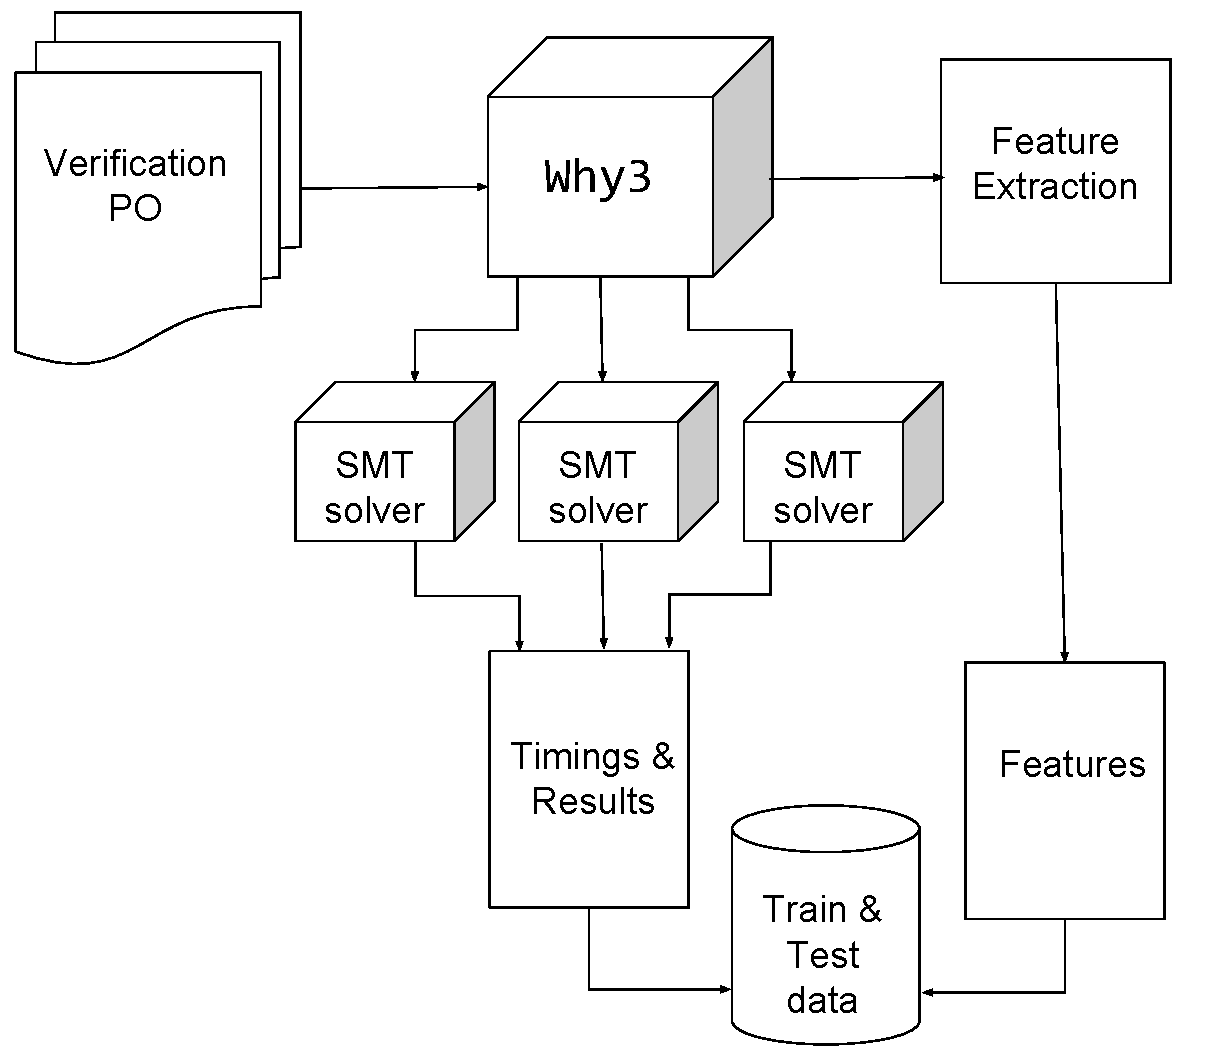
\includegraphics[width=0.9\linewidth]{Figures/Chapter3}
\caption{Diagram illustrating the process to collect predictor and response variables for the \where~model}
\label{fig:Chapter3}
\end{figure}

\section{Selection of tools and programs}
\label{sec:selection}

\subsection{Selection of \why~programs}
\label{sub:why3programs}

As we mentioned in Chapter \ref{LitReview}, \why~was chosen for its modular architecture and ability to read from, and write to, many formats associated with software verification tools. The diversity of input languages in the SV domain was referenced in the previous chapter (Sec. \ref{sub:lrsvmmbench}, \cite{Dagstuhl, deductiveSV}). %Among the input formats which can be parsed by \why are:
%the why intermediate logic format
%
%\begin{itemize}
%	\item \texttt{whyML}: a programming language with support for verification specifications and annotations (native)
%	\item \texttt{why}: the intermediate logic language (native)
%	\item \texttt{TPTP}: the  
%	\item \texttt{Dimacs}: A standard input format for SAT solvers
%\end{itemize} 
We refer the reader to the summary of major benchmark repositories for SV tools given in Table \ref{table:benchmarks}. 
Given the lack of a large standard benchmark repository for software verification systems, we chose to make use of the 128 example programs written in the WhyML programming language as our corpus for training and testing purposes. 
%The programs contain solutions to challenges from the VerifyThis competition and the VACID-0 benchmarks.
These programs are distributed with the \why~software; we used version 0.87.1. 
Many of the programs are solutions to problems posed at software verification competitions such as VerifyThis \cite{verifythis}, VSTTE \cite{Klebanov2011} and COST \cite{bormer:hal-00789525}. 
Other programs are implementations of benchmarks proposed by the VACID-0 \cite{Leino10vacid-0:verification} initiative.   

It is our assumption that the \why~examples are representative of software verification workload. Two alternatives to this dataset are the TPTP \cite{TPTP} library and the BWARE \cite{Delahaye2014} collection of industrial proof obligations. The latter dataset consists of Atelier-B  POs translated into the TPTP format \cite{atelierB2w}. Both these datasets are not specific to the software verification domain: they include scheduling, hardware verification and numerical problems in addition to typical SV tasks. The TPTP repository is limited to first-order logic problems: inductive problems cannot be expressed. The BWARE SMT-LIB translation uses an upper-bound logic of UFNIA -- this set of theories does not use arrays or real arithmetic\footnote{More information about the SMT-LIB standard for logical theories can be found at \url{http://smtlib.cs.uiowa.edu/logics.shtml} }. Both datasets are, however, much larger. The TPTP library currently consists of 20,306 POs \cite{TPTPsite} -- many of which are very similar to each other. There are 12,876 BWARE benchmarks. In comparison, the 128 WhyML programs produced 1048 individual proof obligations. 

The TIP benchmarks \cite{Claessen2015}, while interesting, were not considered as they only measure one aspect of a set of SV tools: their ability to discharge proof obligations which require the use of induction. 

Importantly, the chosen dataset makes use of the full capabilities of the \why~system: the programs include inductive problems and require the use of as many logical theories as each individual SMT solver can reason with.   

\subsection{Selection of \textsc{SMT} solvers}
\label{sub:smtselection}

We used six current, general-purpose SMT solvers supported by \textsf{Why3}: 
\begin{itemize}
	\item \textbf{Alt-Ergo} is a general-purpose SMT solver written in OCaml (the others in this list are written in C++). It is the most tightly-integrated solver supported by \why: it supports polymorphic types and its native input format is a previous version of the \why~intermediate language. Two recent major versions, 0.95.1 and 1.01, are used by \where.
	\item \textbf{CVC3} is the open-source SMT solver developed by the University of Iowa and New York University. We used version 2.4.1.
	\item \textbf{CVC4} is an entirely re-implemented update to CVC3. Version 1.4 is used by \where.
	\item \textbf{veriT} is an open-source SMT solver developed by the University of Lorraine, France, and the Federal University of Rio Grande do Norte, Brazil. We used the current version, 201506, which is not officially supported by \why~v.0.87.1 but is the only version available.
	\item \textbf{Yices} is developed by SRI International and is free for non-commercial use. \where~uses version 1.0.38 rather than Yices2 because the newer implementation does not support quantifiers -- making it unsuitable for SV.  
	\item \textbf{Z3} is the SMT solver developed at Microsoft Research. The source code has been available since 2012 and it has been open-source since 2015. \where~uses two versions: 4.3.2 and 4.4.1. 
\end{itemize}

As Table \ref{table:solvers} shows, the six solvers use four different input formats between them -- three of which are specific to the solver in question. 
This gives some idea of the interoperability capabilities of \why~and the difficulties of comparing tools with a diverse range of input languages. 

Using two versions of Alt-Ergo and Z3 affords the user more flexibility in their local SMT solver installation. 
We describe the process \where~uses to find and use supported SMT solvers on a user's local machine in Chapter~\ref{Implementation}. 

\begin{table}
	\caption[SMT solvers supported by \where]{SMT solvers supported by \where}
 
		\begin{tabularx}{\textwidth}{@{}YYYc@{}}
			\toprule
			\textsc{Solver} &  \textsc{Licence} & \textsc{Why3 driver output} & \textsc{Reference} \\
			%\midrule
			\midrule
			Alt-Ergo & CeCILL-C & \texttt{.why}: Alt-Ergo native input format & \cite{AltErgo} \\ 
			\midrule
			CVC3 & Open-source & \texttt{.cvc}: CVC3 native input format & \cite{CVC3} \\
			\midrule
			CVC4 & BSD & \texttt{.smt}: SMT-LIB version 2 & \cite{CVC4} \\ 
			\midrule
			veriT & BSD & \texttt{.smt}: SMT-LIB version 2 & \cite{veriT} \\
			\midrule
			Yices & Non-commercial use & \texttt{.ycs}: Yices native input format & \cite{Yices} \\
			\midrule
			Z3 & MIT & \texttt{.smt}: SMT-LIB version 2 & \cite{Z3} \\
			\bottomrule	
			
		\end{tabularx}
	
	\label{table:solvers}
\end{table}


\section{Independent/Predictor variables}
\label{sec:independant}

In supervised machine learning terms, these variables represent the known properties of the item from which we want to derive a prediction (in the present case, this item is a computer program). 
The predictor variables must be an accurate characterisation of the program in order for the ML model to be effective. 
We chose to use the proof obligations from goals and lemmas rather than those from axioms and predicates (which tend to be repeated in files using the same logical theories). 
Proof obligations are generated from the goals and lemmas only, while the axioms and predicates provide the context for these POs to be proved by the SMT solver.
%The goals and lemmas are the parts sent to the SMT solver to be proved.   

\subsection{Extracting static metrics from \why~proof obligation formul\ae}
\label{sub:extracting}
%Using the \why notion of "goal shape"

\begin{figure}
	\centering
	\begin{tikzpicture}[
	level 1/.style={sibling distance=30mm},
	edge from parent/.style={->,draw},
	>=latex]
	
	\node[root]{Size}
	child {node[level 2] (c0) {ops}
		child {node[level 2, yshift=10pt] (c1) {divisor}}
		child {node[level 2, yshift=10pt] (c2) {conds}}
	}
	child {node[level 2, yshift=-32pt, xshift=55pt] (c3) {leaves}}
	child {node[level 2, yshift=-32pt, xshift=55pt] (c4) {quants}}
	;
	
	\begin{scope}[every node/.style={level 3}]
	\node [below of = c1, xshift=5pt, yshift=10pt] (c11) {and};
	\node [below of = c11, yshift=10pt] (c12) {or};
	\node [below of = c12, yshift=10pt] (c13) {not};
	\node [below of = c13, yshift=10pt] (c14) {let};
	\node [below of = c14, yshift=10pt] (c15) {as};
	\node [below of = c15, yshift=10pt] (c16) {eps};
	\node [below of = c16, yshift=10pt] (c17) {func};
	
	
	\node [below of = c2, xshift=5pt, yshift=10pt] (c21) {if};
	\node [below of = c21, yshift=10pt] (c22) {iff};
	\node [below of = c22, yshift=10pt] (c23) {imp};
	\node [below of = c23, yshift=10pt] (c24) {case};
	
	
	\node [below of = c3, xshift=5pt, yshift=10pt] (c31) {var};
	\node [below of = c31, yshift=10pt] (c32) {true};
	\node [below of = c32, yshift=10pt] (c33) {false};
	\node [below of = c33, yshift=10pt] (c34) {wild};
	\node [below of = c34, yshift=10pt] (c35) {zero-ar};
	\node [below of = c35, yshift=10pt] (c36) {int};
	\node [below of = c36, yshift=10pt] (c37) {float};
	
	
	\node [below of = c4, xshift=5pt, yshift=10pt] (c41) {forall};
	\node [below of = c41, yshift=10pt] (c42) {exists};
	
	\node [below of = c42](c43) {depth};
	\node [below of = c43](c44) {avg-arity};
	
	\end{scope}
	% lines from each level 1 node to every one of its "children"
	\foreach \value in {1,...,7}
	\draw[->] (c1.195) |- (c1\value.west);
	
	\foreach \value in {1,...,4}
	\draw[->] (c2.195) |- (c2\value.west);
	
	\foreach \value in {1,...,7}
	\draw[->] (c3.195) |- (c3\value.west);
	
	\foreach \value in {1,...,2}
	\draw[->] (c4.195) |- (c4\value.west);
	
	\end{tikzpicture}
	\caption{Tree illustrating the Why syntactic features counted by traversing the AST.}
	\label{fig:types}
\end{figure}

To extract the structural metrics from the logical formul\ae, we traversed the abstract syntax tree (AST) representation. 
We made use of the \why~OCaml API to do this. 
Our approach is similar to the method used internally by \why~to derive a \textit{shape} string from an interactive proof session \cite{why:preserving}. 
The purpose of shape strings in this context is to track changes in the POs and avoid re-proving files unnecessarily. 
The shape acts as a minimal fingerprint representing the structure of the PO formula. 
Instead of producing a string after traversing the AST, our process simply counts the syntactic features of the formula to construct a feature vector.

Fig. \ref{fig:types} lists the predictor variables that were used in our study.  
All of these are (integer-valued) metrics that can be calculated by analysing the \textsf{Why3} goal statement, and are similar to the \textit{Syntax} metadata category for proof obligations written in the TPTP format \cite{TPTP}. 
The metrics we chose to characterise \why~proof obligations are intended to generalise for first-order formul\ae~and other IVLs such as Boogie \cite{Boogie} rather than be specific to \why~syntax.
The metrics' simplicity also makes the ML models more transparent and understandable: metrics derived from multiple complicated interactions of structural features would be hard to reason about and apply to other related contexts where learning would be useful. 

The features shown in pink rectangles in Fig. \ref{fig:types} are counted individually by traversing the AST. 
The rounded blue nodes represent metrics that are the sum of their children in the tree. 
The metrics represented by pink rectangles measure syntactic features and are self-explanatory except for the following:
\begin{itemize}[leftmargin=*]
	\item[] \textbf{zero-ar:} The number of functions which do not take any arguments (i.e. zero-arity functions).
	\item[] \textbf{depth:} The depth of the AST.
	\item[] \textbf{avg-arity:} The total number of arguments for all functions which are children of the \textit{divisor} node, divided by the value of \textit{divisor}.
\end{itemize}   

\textit{Size} measures the size the expression and is the sum of \textit{ops} (the number of operators), \textit{leaves} (the number of leaf nodes in the AST), and \textit{quants} (the number of quantifiers). 
We map our notion of \textit{conds} to the number of decision nodes used to calculate McCabe's cyclomatic complexity metric discussed in Sec. \ref{sec:lrmm}.
  

\subsubsection{Example: \textit{first\_last} lemma}

As a minimal illustrative example, we refer to the code listing in Fig. \ref{fig:code}. 
This code is one of the 13 POs from the \texttt{edit\_distance.mlw} file in the \why~examples directory. 
The entire program verifies an algorithm which finds the ``edit distance''\footnote{\url{https://en.wikipedia.org/wiki/Edit_distance}} similarity measure between two strings.  
Informally, this intermediate lemma asserts that the same words are produced by (i) prepending a word (minus its first letter \textit{a}) with \textit{a} and (ii) appending a word (minus its last letter \textit{b}) with \textit{b}. 
A representation of the parse tree from this lemma is shown in Fig. \ref{fig:tree}. 
The root node (\textit{forall}) is circled and the leaf nodes are shown as rectangles.
The name of each \textit{func} (as interpreted by \why) is shown for clarity.
The reader will note that the zero-arity function \textit{Nil} is a leaf node in the tree, while all other functions (\textit{Cons, =, ++, length}) and operators (\textit{and}) have an arity of either 1 or 2. 

Table \ref{table:examplemetrics} shows the non-zero metrics used to describe the \textit{first\_last} formula for predictive purposes.

\begin{figure}
	\centering 
	\lstinputlisting[language=ML, firstline=60, lastline=62]{edit_distance.txt}
	\caption{ \textit{WhyML} code for the \textit{first\_last} lemma in \textit{edit\_distance.mlw}}
	\label{fig:code}
\end{figure}

\begin{figure}
	\centering
	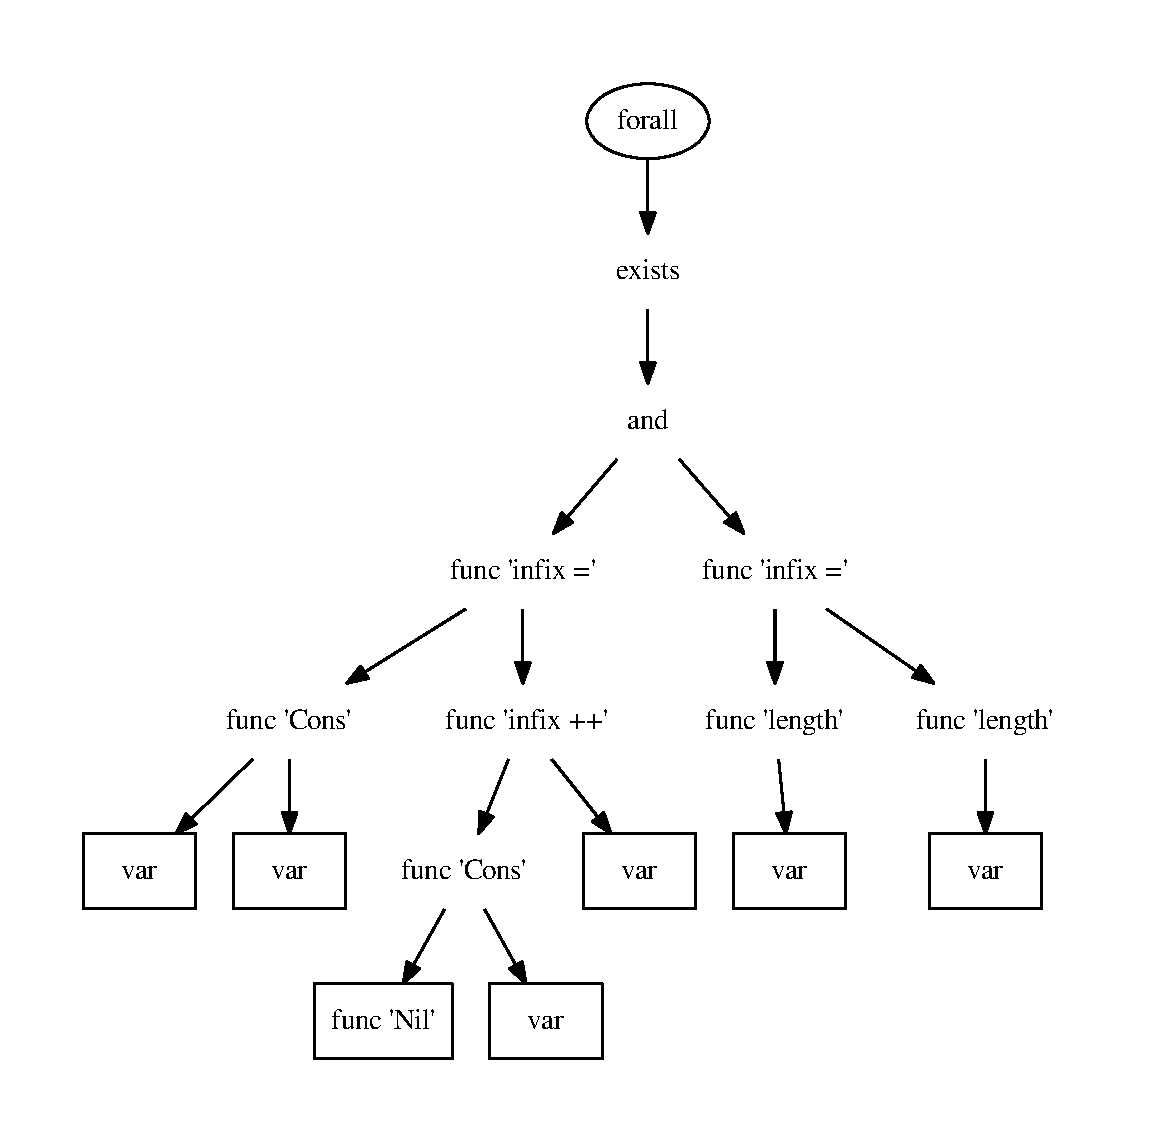
\includegraphics[width=0.9\textwidth]{code}
	\caption{The parse tree extracted from the \textit{first\_last} goal (Fig. \ref{fig:code})}
	\label{fig:tree}
\end{figure}

%%

% 	"and": 1.0,
% 	"exists": 1.0,
% 	"n_quants": 2.0,
% 	"zero_ar": 1.0,
% 	"n_branches": 7.0,
% 	"n_ops": 9.0,
% 	"var": 6.0,
% 	"size": 17.0,
% 	"avg_op_arity": 1.55
% 	"forall": 1.0,
% 	"func": 8.0,
% 	"divisor": 9.0,
% 	"depth": 7.0,

%% 

\begin{table}
	\centering
	\caption{Non-zero metrics calculated for \textit{first\_last}} 
	\label{table:examplemetrics}
	\begin{tabular}
		{|r|r|c|r|r|c|r|r|} \hline
		Metric&Value&&Metric&Value&&Metric&Value \\ \hline
		\texttt{and}&1&&\texttt{exists}&1&&\texttt{forall}&1 \\ \hline
		\texttt{var}&6&&\texttt{func}&8&&\texttt{quants}&2 \\ \hline
		\texttt{ops}&9&&\texttt{leaves}&7&&\texttt{depth}&7 \\ \hline
		\texttt{size}&17&&\texttt{divisor}&9&& \texttt{avg\_arity}&1.55 \\ 
		\hline
		\texttt{zero\_ar}&1&& & && & \\ \hline	
	\end{tabular}
\end{table}


\section{Dependent/Response variables}
%Measurement of dynamic properties
\label{sec:dependant}

Our evaluation of the performance of a solver depends on two factors: the time taken to calculate the result, and the solver's output as interpreted by \why.

\subsection{Execution time}
%mention the rationale behind choosing 10 seconds as a reasonable time limit   
In order to accurately measure the time each solver takes to return an answer, we used a measurement framework specifically designed for use in competitive environments. 
The BenchExec \cite{ Beyer2016,benchexec} framework was developed by the organisers of the SV-COMP \cite{SVCOMP} software verification competition to reliably measure CPU time, wall-clock time and memory usage of software verification tools. 
We recorded the time spent on CPU by each SMT solver for each proof obligation. 

\subsubsection{Accounting for randomness with confidence intervals}
\label{sub:confidence}

Any effort to measure execution time accurately is hampered by random errors introduced by the experimental environment.
To account for these errors, we used the methodology described by Lilja \cite{LiljaJ} to obtain an approximation of the true mean execution time. 

As each solver execution can be quite expensive in terms of time (a worst case scenario for one measurement of each PO: 1048 (POs) $\times$ 8 (solvers) $\times$ 10 seconds (time limit) $\approxeq$ 23.3 hours of computation time), a small number of initial measurements (five) were made.
From these sample measurements, the mean execution time $\bar{x}$ and standard deviation $s$ were computed. 
To determine the number of measurements ($n$) required for a statistically-significant sample, we assume that the random errors have a $Student's$ $t$-distribution (similar in shape to a Gaussian distribution). 
We can use these measurements to find the confidence interval $(c_1, c_2)$ using the equations:
\begin{equation}
	c_1=(1-e)\bar{x} = \bar{x}-z_{1-a/2;n-1}\frac{s}{\sqrt{n}} 
	\label{eq:c1}
\end{equation}
\begin{equation}
	c_2=(1+e)\bar{x} = \bar{x}+z_{1-a/2;n-1}\frac{s}{\sqrt{n}}
	\label{eq:c2}
\end{equation}
Either Equation \ref{eq:c1} or \ref{eq:c2} can be used to find 
\begin{equation}
	z_{1-a/2}\frac{s}{\sqrt{n}} = \bar{x}e.
	\label{eq:simp}
\end{equation}
Solving for $n$ gives
\begin{equation}
	n =
	 \left(\frac{z_{1-a/2}s}{e\bar{x}}\right)^2
	\label{eq:n}
\end{equation}
  
where $z$ is a value from the $t$-distribution which is used to model the measurement error. 
An illustration of this distribution, Fig. \ref{fig:confidence}, shows that there is a probability $1-a$ that the actual value being measured (i.e. \textit{x}: the execution time for each solver to return an answer for a particular PO), is within the confidence interval ($c_1, c_2$). 
As the bounds of ($c_1, c_2$) increase outward, the confidence level increases.
We can be 100\% confident that the actual mean value is within the interval (0, $\infty$) but this interval is not practical.  
A value of 0.1 was chosen for \textit{a}, meaning we can be 90\% confident that the actual value of \textit{x} is between $c_1$ and $c_2$. 
We allow the computed mean value to be within 7\% of the actual mean (i.e. seven degrees of freedom or an allowed error of $\pm$3.5\%). Thus for the equations \ref{eq:c1} to \ref{eq:n}, we take $e = 0.035$.  \\ 
\\
\textbf{Example: finding Alt-Ergo's execution time for \textit{first\_last}}: \\
To show how this method is used in practice, we return to the example introduced in Sec. \ref{sub:extracting} -- the \textit{first\_last} goal from \textbf{edit\_distance.mlw}'s \textbf{Word} theory.
The five sample measurements of CPU time spent by Alt-Ergo (to return an answer of \textit{Unknown}):

\begin{tabularx}
	{\textwidth}{@{}YYYYY@{}}
	 $\lbrace$ 0.124, & 0.142, & 0.136, & 0.131, & 0.133 $\rbrace$
\end{tabularx} 

given a sample mean ($\bar{x}$) and sample standard deviation ($s$) of 0.133 and 0.006 respectively. 
Consulting a table for the $t$ distribution, we find that when $a=0.1$ and we require seven degrees of freedom, $t_{0.95;7} = 1.895$.
Substituting these values into equation \ref{eq:n}, we find
\begin{equation}
	n =  \left(\frac{z_{1-a/2}s}{e\bar{x}}\right)^2
	= \left(\frac{1.895(0.006)}{0.035(0.133)}\right)^2 = 5.966
\end{equation}    
Therefore, we need to make six measurements to be assured that there is a 90\% chance that the true value is within this $\pm3.5\%$ interval.

For completeness, the extra measurement yielded a value of 0.135; making the CPU time Alt-Ergo spent solving \textit{first\_last} the mean of the six measurements: 0.134 seconds.

\begin{figure}
\centering
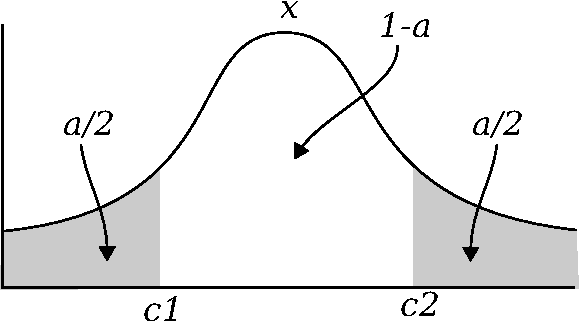
\includegraphics[width=0.6\linewidth]{Figures/confidence}
\caption[Accounting for errors in measurement of solver execution time \textit{x}]{Accounting for errors in measurement of solver execution time \textit{x}}
\label{fig:confidence}
\end{figure}


%By inspecting our data, we saw that most \textit{Valid} and \textit{Invalid} answers returned very quickly, with \textit{Unknown} answers taking slightly longer, and \textit{Failure/Timeout} responses taking longest. We took the relative utility of responses to be $Valid >$ $Invalid>Unknown>Timeout>Failure$ which can be read as ``it is better for a solver to return a \textit{Valid} response than \textit{Timeout}'', etc. A simple function allocates a cost to each solver $S$'s response to each goal $G$:
%\[\small
%cost(S,G) = 
%\begin{cases}
%time_{S,G}, \text{ if answer}_{S,G} \in \lbrace Valid, Invalid \rbrace \\
%time_{S,G} + \text{timeout}, \text{ if answer}_{S,G} = Unknown \\
%dist((time_{S,G},\text{timeout}), (0,0)), \text{if answer}_{S,G} \in \lbrace Timeout, Failure \rbrace
%\end{cases}
%\]
%
%Thus, to penalise the solvers that return an \textit{Unknown} result, the timeout limit is added to the time taken, while solvers returning \textit{Timeout} or \textit{Failure} are further penalised by taking the Euclidean distance from $(0,0)$ to the point defined by the (time taken, timeout limit). This function ensures the best-performing solvers always have the lowest costs. A ranking of solvers for each goal in order of decreasing relevance is obtained by sorting the solvers by ascending cost.
%
%Since our cost model depends on the timeout value chosen, we need to choose a value that does not favour any one solver.  To establish a realistic timeout limit, we find each solver's ``Peter Principle Point'' \cite{Sutcliffe200139}. In resource allocation for theorem proving terms, this point can be defined as the time limit at which more resources will not lead to a significant increase in the number of goals the solver can prove. 

\subsection{Prover output}
\label{sub:prover-output}

\begin{figure}
	\centering
	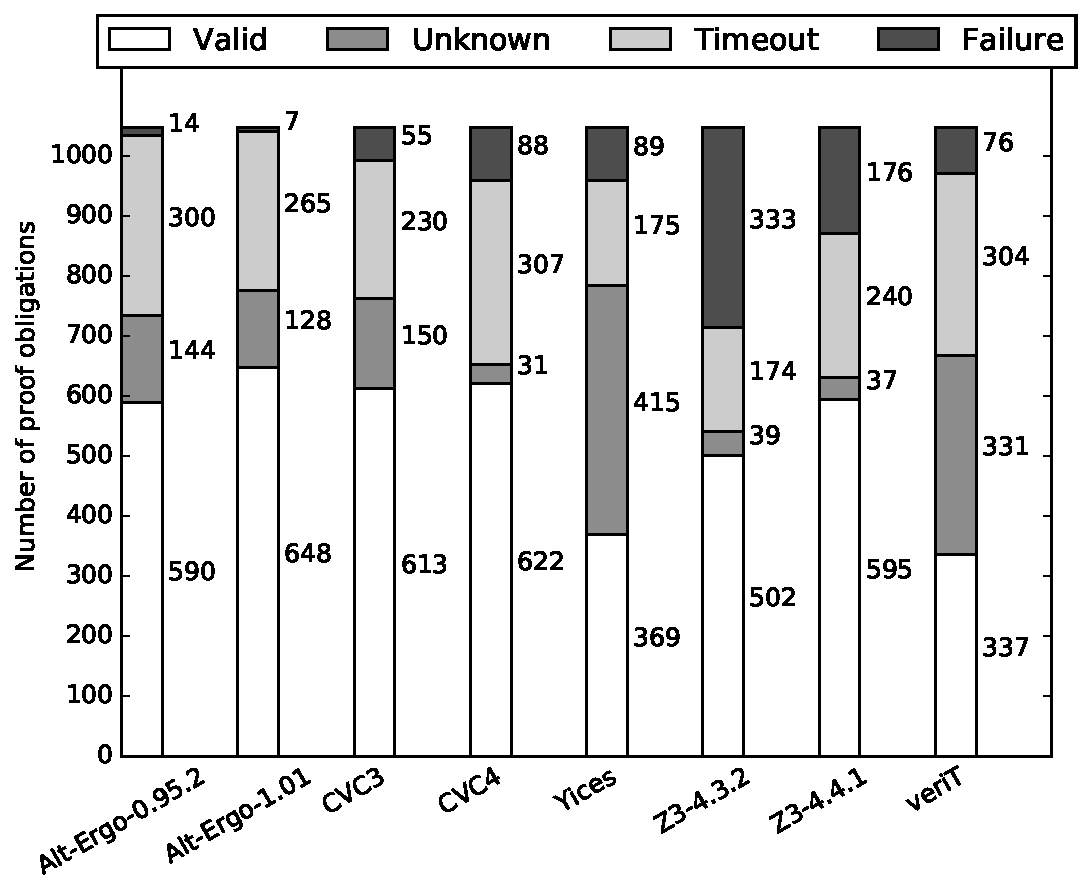
\includegraphics[width=0.8\linewidth]{barcharts}
	\caption[The relative amount of Valid / Unknown / Timeout / Failure answers from the eight SMT solvers]{The relative amount of Valid / Unknown / Timeout / Failure answers from the eight SMT solvers (with a timeout of 60 seconds). }
	\label{fig:barcharts}
\end{figure}


When a solver is sent a goal by \why, it returns an answer $A$ where $A$ is one of $\lbrace Valid,Invalid,Unknown,Timeout,Failure \rbrace$. The following definitions of these answers are taken from the \why~User Manual \cite{why:manual}.\\  

\begin{tabularx}
	{\textwidth}{@{}ll@{}}
	\textbf{Valid}   & The goal is proved in the given context. \\
	\textbf{Invalid} & The prover knows the goal cannot be proved. \\  
	\textbf{Unknown} & The prover has stopped its search.\\
	\textbf{Timeout} & The prover has reached the time limit. \\
	\textbf{Failure} & An error has occurred. \\
\end{tabularx}\\

Fig. \ref{fig:barcharts} shows the relative amount of $Valid / Unknown / Timeout / Failure$ answers from the eight SMT solvers (when given a timeout of 60 seconds) on the entire dataset of 1048 POs. 
For example, Alt-Ergo version 0.95.1 (leftmost bar) returned an answer of \textit{Valid} for 590 POs, \textit{Unknown} for 144 POs, \textit{Timeout} for 300, and \textit{Failure} for 14.
Note that no tool returned an answer of Invalid for any of the 1048 proof obligations.
We assume this is because the example programs are verified algorithms/data-structures and an answer of \textit{Invalid} would indicate a violated pre-/post- condition or invariant.
The limitations of our chosen dataset and other threats to validity are discussed later in the thesis (Sec. \ref{sec:threats}).

Often, goals that cannot be proved \textit{Valid} or \textit{Invalid} require inductive reasoning through the use of an interactive theorem prover such as Isabelle \cite{Isabelle} or Coq \cite{Coq}. 
Sometimes a splitting transformation needs to be applied in order to simplify the goals before they are sent to the solver. 
\where~does not perform any transformations to goals other than those defined by the solver's \why~driver file. 
In other cases, more time or memory resources need to be allocated in order to return a conclusive result. 
We address the issue of resource allocation in the next subsection.    

\subsubsection{Setting a timeout limit for measurement}
\label{sub:timeout-limit}

\begin{figure}
	\centering
	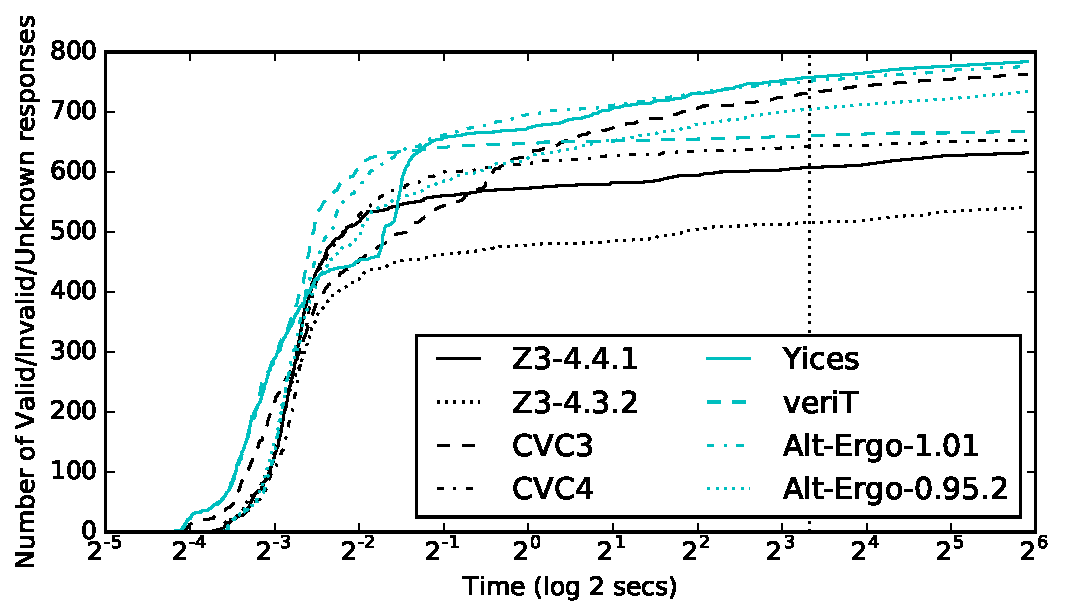
\includegraphics[width=\linewidth]{line_graph}
	\caption[Cumulative number of useful responses for each solver over 60 seconds]{The cumulative number of \textit{Valid/Invalid/Unknown} responses for each solver for the entire dataset of 1048 POs. The plot uses a logarithmic scale on the time axis for increased clarity at the low end of the scale.}
	\label{fig:line_graph}
\end{figure}

\sloppypar
A solver is said to return a \textit{useful} result if it returns an answer of \textit{Valid}, \textit{Invalid} or \textit{Unknown} when given a reasonable timeout limit.
We justify this statement by making the observation that an answer of \textit{Failure} usually means there is an error in logical translation of the PO. 
The failing solver is not a good choice for the particular logics required to return a \textit{Valid} or \textit{Invalid} answer.
\textit{Unknown} answers are usually identified as such very quickly therefore they do not impose a long waiting period for an answer and \where~can call another solver with a minimal delay.
By definition, \textit{Timeout} results incur the maximal time penalty.  
    
Fig. \ref{fig:line_graph} shows the number of \textit{Valid/Invalid/Unknown} results for each solver when given a timeout value of 60 seconds. 
For example, the solid black line shows the useful results for version 4.4.1 of Z3.
At $2^{-3}$ (0.125) seconds, Z3 returned 130 \textit{Valid/Invalid/Unknown} results. 
This number increases sharply to 518 after $2^{-2}$ (0.25) seconds, before levelling off.
If Z3 is given a time limit of 60 seconds, only 125 more useful responses are returned; giving a total of 632.  

The value of 60 seconds was chosen as an upper limit, since this timeout value is not realistic for most software verification scenarios.  
\why, for example, has a default timeout value of five seconds.
By inspecting the plot of solver answers in Fig. \ref{fig:line_graph}, we can see that the number of useful answers returned levels off very quickly. 
From this observation we deduce that the likelihood of a \textit{Timeout} answer potentially turning into a \textit{Valid/Invalid} answer (if given more time) is minimal.  
%From Fig. \ref{fig:line_graph} we can see that the vast majority of useful responses are returned very quickly. 

To establish a realistic timeout limit, we find each solver's ``Peter Principle Point'' \cite{Sutcliffe200139}. In resource allocation for theorem proving terms, this point can be defined as the time limit at which more resources will not lead to a significant increase in the number of goals the solver can prove.
By satisfying ourselves with being able to record 99\% of the useful responses which would be returned after 60 seconds, a more reasonable threshold is obtained for each solver. 
To calculate this time value for each solver, we find the time at which 99\% of the solver's total number of \textit{Valid / Invalid / Unknown} responses have be returned. 
This threshold ranges from 7.35 secs (veriT) to 9.69 secs (Z3-4.3.2). Thus we chose a value of ten seconds (Fig. \ref{fig:line_graph}'s \textit{dotted vertical line}) as a representative, realistic timeout that gives each solver a fair opportunity to return decent results.     



\section{Summary}

In this chapter, we have introduced the SMT solvers, training and testing dataset, predictor and response variables used by the \where~model.
The choices made in regard to the SMT solvers were dictated to a large extent by \why~and its selection of drivers. 
The dataset contains solutions to canonical SV challenges and is designed to demonstrate the specification and verification of data structures and algorithms fundamental to a wide range of applications, using the full capabilities of the \why~system.
The choice of predictor variables was influenced by the structural metrics introduced by McCabe (see Sec. \ref{sec:lrmm}), which have become established in the SE domain, and syntactic features similar to those used in TPTP library metadata. 
The response variables of \textit{time} and \textit{result} are similar to the scoring mechanism used for SV tools in the SV-COMP \cite{SVCOMP}.
The response variables will be combined in the next chapter as a single value suitable for prediction by a variety of regression models.

After conducting the data preparation discussed in this chapter, we have collected particular information about each proof obligation: 
\begin{itemize}
	\item the time each of the eight solvers takes to return an answer when given a time limit value of ten seconds
	\item each solver's response (\textit{Valid/Timeout/etc.}) for the same time limit
	\item a feature vector consisting of the twenty-eight structural and syntactic metrics listed in Fig. \ref{fig:types} 
\end{itemize}   
The material presented in this chapter is critical to how the \where~model functions and forms the basis for the experiments presented in the next chapter. 
  


